% ОБЯЗАТЕЛЬНО ИМЕННО ТАКОЙ documentclass!
% (Основной кегль = 14pt, поэтому необходим extsizes)
% Формат, разумеется, А4
% article потому что стандарт не подразумевает разделов
% Глава = section, Параграф = subsection
% (понятия "глава" и "параграф" из документа, описывающего диплом)
\documentclass[a4paper,14pt]{extarticle}

% Подключаем главный пакет со всем необходимым
\usepackage{diploma}

% Пакеты по желанию (самые распространенные)
% Хитрые мат. символы
\usepackage{euscript}
% Таблицы
\usepackage{longtable}
\usepackage{makecell}
% Картинки (можно встявлять даже pdf)
\usepackage[pdftex]{graphicx}

\usepackage{amsthm,amssymb, amsmath}
\usepackage{textcomp}

% Подсветка кода (все стили в файле)
\usepackage{color}
\usepackage{listings}
\definecolor{GrayCodeBlock}{RGB}{248,252,255}
\definecolor{BlackText}{RGB}{41,75,102}
\definecolor{RedTypename}{RGB}{182,86,17}
\definecolor{GreenString}{RGB}{96,172,57}
\definecolor{PurpleKeyword}{RGB}{184,84,212}
\definecolor{GrayComment}{RGB}{100,100,100}
\definecolor{GoldDocumentation}{RGB}{180,165,45}

\lstset{
    columns=fullflexible,
    keepspaces=true,
    frame=single,
    framesep=0pt,
    framerule=0pt,
    framexleftmargin=4pt,
    framexrightmargin=4pt,
    framextopmargin=5pt,
    framexbottommargin=3pt,
    xleftmargin=4pt,
    xrightmargin=4pt,
    backgroundcolor=\color{GrayCodeBlock},
    basicstyle=\ttfamily\small\color{BlackText},
    keywordstyle=\color{PurpleKeyword},
    ndkeywordstyle=\color{RedTypename},
    comment=[l][\color{GrayComment}\slshape]{//},
    morecomment=[s][\color{GrayComment}\slshape]{/*}{*/},
    morecomment=[s][\color{RedTypename}]{\#![}{]},
    morecomment=[s][\color{RedTypename}]{\#[}{]},
    stringstyle=\color{GreenString},
    string=[b]"
}

\lstdefinelanguage{rust}
{
    keywords={
        true,false,
        unsafe,async,await,move,
        use,pub,crate,super,self,mod,
        struct,enum,fn,const,static,let,mut,ref,type,impl,dyn,trait,where,as,
        break,continue,if,else,while,for,loop,match,return,yield,in
    },
    ndkeywords={
        bool,u8,u16,u32,u64,u128,i8,i16,i32,i64,i128,char,str,
        Self,Option,Some,None,Result,Ok,Err,String,Box,Vec,Rc,Arc,Cell,RefCell,HashMap,BTreeMap,
        macro_rules
    },
    comment=[l][\color{GrayComment}\slshape]{//}
}


\begin{document}

% Титульник в файле titlepage.tex
\newgeometry{left=30mm, top=20mm, right=15mm, bottom=20mm, nohead, nofoot}
\begin{titlepage}
\begin{center}

Федеральное государственное автономное \\образовательное учреждение высшего образования

\textbf{<<Национальный исследовательский ядерный университет}
\textbf{<<МИФИ>>}

\vspace{35mm}

\textbf{\textit{\large Музыкина Екатерина Андреевна}} \\[8mm]
% Название
\textbf{\large Выпускная квалификационная работа}\\[3mm]
\textbf{\textit{\large Название работы}}

\vspace{20mm}
Уровень образования: магистратура\\
Направление 11.04.04 «Электроника и наноэлектроника»\\
Образовательная программа
«Наноэлектроника, спинтроника и фотоника»\\[25mm]


% Научный руководитель, рецензент
\begin{flushright}
\begin{minipage}[t]{0.5\textwidth}
{Научный руководитель:} \\
к.ф.-м.н., доцент кафедры \\физики конденсированных сред, \\ Сибирмовский Ю.Д.

\vspace{10mm}

{Рецензент:} \\
 \\
\end{minipage}
\end{flushright}

\vfill 

{Москва}
\par{\the\year{} г.}
\end{center}
\end{titlepage}
% Возвращаем настройки geometry обратно (то, что объявлено в преамбуле)
\restoregeometry
% Добавляем 1 к счетчику страниц ПОСЛЕ titlepage, чтобы исключить 
% влияние titlepage environment
\addtocounter{page}{1}


% Содержание
\tableofcontents
\pagebreak

% ============================================
% ВВЕДЕНИЕ
% ============================================
\specialsection{Введение}

Здесь необходимо рассказать, о чём работа. Объём 1-2 страницы. Нужно охарактеризовать область исследования, практическую значимость (для разработки каких приборов могут быть использованы ваши результаты), какую проблему решает ваша работа (кратко, подробнее будет в обзоре), какие методы использованы (тоже кратко, подробнее в главе Методы).

Здесь необходимо рассказать, о чём работа. Объём 1-2 страницы. Нужно охарактеризовать область исследования, практическую значимость (для разработки каких приборов могут быть использованы ваши результаты), какую проблему решает ваша работа (кратко, подробнее будет в обзоре), какие методы использованы (тоже кратко, подробнее в главе Методы).

Здесь необходимо рассказать, о чём работа. Объём 1-2 страницы. Нужно охарактеризовать область исследования, практическую значимость (для разработки каких приборов могут быть использованы ваши результаты), какую проблему решает ваша работа (кратко, подробнее будет в обзоре), какие методы использованы (тоже кратко, подробнее в главе Методы).

\specialsection{Цель и задачи}
\label{Tasks}

\textbf{Цель:} Цель не должна совпадать с темой работы. Цель должна быть достижима (должен быть конечный результат) и проверяема. Исследование --- это процесс, и целью быть не может.

\textbf{Задачи}
\begin{enumerate}
    \item Задача 1
    \item Задача 2
    \item Задача 3
    \item Задача 4
\end{enumerate}

Достаточно задач. Обзор литературы наверное в задачи включать не будем. Лучше написать конкретно, что мы делаем (разработка алгоритма, программная реализация, расчёт конкретных параметров при определённых условиях и т.д.)

% ============================================
% ГЛАВА 1
% ============================================
\pagebreak
\section{Обзор литературы}

\subsection{Раздел 1}

\begin{figure}[ht]
    \begin{center}
    \scalebox{0.4}{
       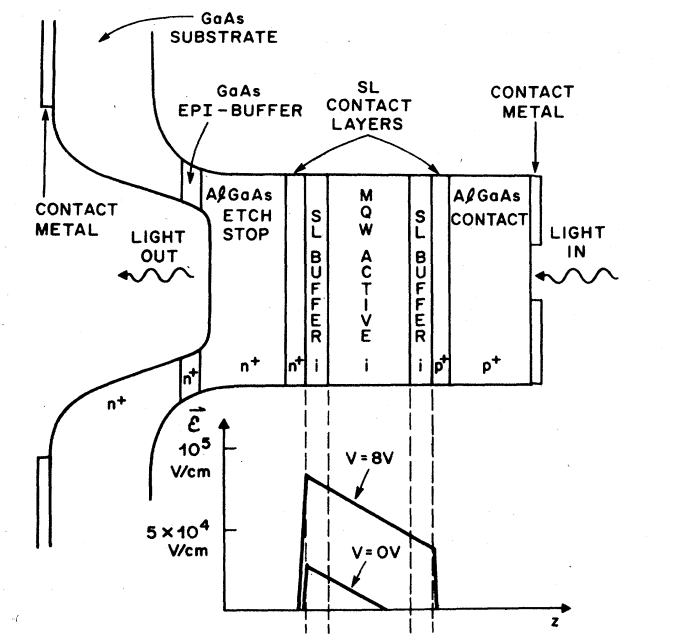
\includegraphics{images/Miller2-Figure2.png}
    }
    
    \caption{\label{fig:miller2-2}
        Схема измерений спектров поглощения в поперечном поле из работы \cite{Miller2}.}
    \end {center}
    \end {figure}
    
    Если рисунок взят из какой-то статьи, книги или из интернета (из интернета нежелательно), то нужно обязательно в подписи сделать ссылку на соответствующий пункт в списке литературы.

    Ссылаемся на рисунок \ref{fig:miller2-2}.
    
    Ссылка на статью: \cite{Miller2}, \cite{Mohseni}

\subsection{Раздел 2}

% ============================================
% ГЛАВА 2
% ============================================
\pagebreak
\section{Теория и основные уравнения}

\subsection{Раздел 1}

Ненумерованная формула:

\begin{equation}
    \begin{pmatrix} \dot{\varphi}\\ \dot{\theta} \\ \dot{\psi} \end{pmatrix}
    = \begin{pmatrix}
        cos(\theta)cos(\psi) & -sin(\psi) & 0 \\
        cos(\theta)sin(\psi) & cos(\psi)  & 0 \\
        -sin(\theta)         & 0         &  1
    \end{pmatrix}^{-1}
    \begin{pmatrix} \omega_x\\ \omega_y \\ \omega_z \end{pmatrix}.
\end{equation}

\subsection{Раздел 2}

Нумерованная формула:

\begin{equation}
    i^2 = -1.
    \label{eq:my_ref}
\end{equation}

Тест ссылки на формулу \ref{eq:my_ref}.

% ============================================
% ГЛАВА 3
% ============================================
\pagebreak
\section{Численные методы и алгоритмы}

\subsection{Раздел 1}

\subsection{Раздел 2}

% ============================================
% ГЛАВА 4
% ============================================
\pagebreak
\section{Программная реализация}

\begin{lstlisting}[language=rust,caption={Программная реализация метода Рунге-Кутты},label={listing-1}]
    // From the pendulum program
    fn runge_kutta(
        vars: &MyVec,
        pars: &Vec<f64>,
        rhs: &dyn Fn(&MyVec, &Vec<f64>) -> MyVec,
        dt: f64,
    ) -> MyVec {
        let rk_1 = rhs(vars, pars);
        let rk_2 = rhs(&vars.add(&rk_1.scale(dt / 2.0)), pars);
        let rk_3 = rhs(&vars.add(&rk_2.scale(dt / 2.0)), pars);
        let rk_4 = rhs(&vars.add(&rk_3.scale(dt)), pars);
    
        let vars_new = vars
            .add(&rk_1.scale(dt / 6.0))
            .add(&rk_2.scale(dt / 3.0))
            .add(&rk_3.scale(dt / 3.0))
            .add(&rk_4.scale(dt / 6.0));
        vars_new
    }
    \end{lstlisting}
    
    \begin{lstlisting}[language=C++,caption={Подпрограмма случайного блуждания на плоскости},label={listing-2}]
    std::random_device rd;
    std::mt19937 mt(rd());
    std::uniform_int_distribution<long> dist(1, 4);
    std::vector<long> xn(n0, 0);
    std::vector<long> yn(n0, 0);
    for (long jt = 0; jt < M; jt++)
    {
        for (long jn = 0; jn < n0; jn++)
        {
            switch (dist(mt))
            {
            case 1:
                xn[jn] ++;
                break;
            case 2:
                xn[jn] --;
                break;
            case 3:
                yn[jn] ++;
                break;
            case 4:
                yn[jn] --;
                break;
            }
        }
    }
    \end{lstlisting}

% ============================================
% ГЛАВА 5
% ============================================
\pagebreak
\section{Результаты и обсуждение}

Ниже тестируется очень большая таблица на несколько страниц

\begin{center}
    \begin{longtable}{|p{2cm}|p{3cm}|p{7cm}|p{3cm}|}
    \caption{Заголовок таблицы}\\
    \hline
    1 & 2 & 3 & 4\\ 
    \hline 
    2 & 2 & 3 & 4\\
    \hline
    3 & 2 & 3 & 4\\
    \hline
    4 & 2 & 3 & 4\\
    \hline
    5 & 2 & 3 & 4\\
    \hline
    6 & 2 & 3 & 4\\
    \hline
    7 & 2 & 3 & 4\\
    \hline
    8 & 2 & 3 & 4\\
    \hline
    9 & 2 & 3 & 4\\
    \hline
    10 & 2 & 3 & 4\\
    \hline
    
    
    \end{longtable}
\end{center}


А также тестируется счетчик таблиц, жирные и двойные линии.

\begin{center}
    \begin{longtable}{|p{2cm}||p{3cm}|p{7cm}|p{3cm}|}
    \caption{Заголовок таблицы нумер 2}\\
    \hline
    1 & 2 & 3 & 4\\ 
    \hline
    2 & 2 & 3 & 4\\
    \hline
    3 & 2 & очень жирная ячейка \par с переносом & 4\\
    \hline
    4 & 2 & 3 & 4\\
    \hline
    5 & 2 & 3 & 4\\
    \hline
    6 & 2 & 3 & 4\\
    \hline
    7 & 2 & 3 & 4\\
    \hline
    8 & 2 & 3 & 4\\
    \hline
    9 & 2 & 3 & 4\\
    \hline
    10 & 2 & 3 & 4\\
    \hline
    
    
    \end{longtable}
\end{center}

Ссылаемся на Листинг \ref{listing-1} здесь.

% ============================================
%  ВЫВОДЫ И ЗАКЛЮЧЕНИЕ
% ============================================
\pagebreak
\specialsection{Выводы}
Жизнь --- тлен.

\specialsection{Заключение}
Нужны ли отдельно и выводы, и заключение --- я не знаю. Разберёмся.

Список литературы ниже оформлен не по ГОСТу, но это легко исправить. Главное, что он организован, и можно ссылаться на каждый пункт по фамилии первого автора. Так же надо сделать и вам.

\begin{thebibliography}{99}

    \bibitem{Miller0} D.A.B. Miller, D. S. Chemla, T. C. Damen et al., Band-Edge Electroabsorption in Quantum Well Structures: The Quantum-Confined Stark Effect, Phys. Rev. Lett., 53 (1984), 2173. \url{https://doi.org/10.1103/PhysRevLett.53.2173}

    \bibitem{Miller1} D.A.B. Miller, D.S. Chemla, T.C. Damen et al., Electric Field Dependence of Optical Absorption near the Band Gap of Quantum-Well Structures, Phys. Rev. B, 32, 2 (1985), 1043–60. \url{https://doi.org/10.1103/PhysRevB.32.1043}
    
    \bibitem{Miller2} D. Miller, J. Weiner, D. Chemla et al., Electric-field dependence of linear optical properties in quantum well structures: Waveguide electroabsorption and sum rules, IEEE J. Quantum Electronics, 22, 9 (1986), 1816-1830. \url{https://doi.org/10.1109/JQE.1986.1073167}
    
    \bibitem{Klipstein} P.C. Klipstein and N. Apsley, A theory for the electroreflectance spectra of quantum well structures. J. Phys. C: Solid State Phys., 19 (1986), 6461. \url{https://doi.org/10.1088/0022-3719/19/32/020}
    
    \bibitem{Kan} Kan, Y., H. Nagai, M. Yamanishi et al., Field Effects on the Refractive Index and Absorption Coefficient in AlGaAs Quantum Well Structures and Their Feasibility for Electrooptic Device Applications, IEEE J. Quant. Electronics, 23, 12 (1987), 2167–80. \url{https://doi.org/10.1109/JQE.1987.1073288}
    
    \bibitem{Weiner} J.S. Weiner, D.A.B. Miller and D.S. Chemla, Quadratic electro-optic effect due to the quantum-confined Stark effect in quantum wells, Appl. Phys. Lett., 50 (1987), 842-844. \url{https://doi.org/10.1063/1.98008}
    
    \bibitem{Mohseni} H. Mohseni, H. An, Z. A. Shellenbarger, M. H. Kwakernaak, and J. H. Abeles, Enhanced Electro-Optic Effect in GaInAsP-InP Three-Step Quantum Wells, Appl. Phys. Lett., 84, 11 (2004), 1823–25. \url{https://doi.org/10.1063/1.1682699}
    
    \bibitem{Arakawa} T. Arakawa, T. Toya, M. Ushigome et al., InGaAs/InAlAs five-layer asymmetric coupled quantum well exhibiting giant electrorefractive index change, Jap. J. Appl. Phys., 50 (2011), 032204. \url{https://doi.org/10.1143/JJAP.50.032204}
    
    \bibitem{Dave} D.P. Dave, Enhanced Refractive Index Change in Asymmetrical Quantum Wells with an Applied Electric Field, J. Appl. Phys., 74, 11 (1993), 6872–75. \url{https://doi.org/10.1063/1.355089}
    
    \bibitem{Feng} H. Feng, J.P. Pang, M. Sugiyama et al., Field-Induced Optical Effect in a Five-Step Asymmetric Coupled Quantum Well with Modified Potential, IEEE J. Quant. Electronics, 34, 7, (1998), 1197-1208. \url{https://doi.org/10.1109/3.687863}
    
    \bibitem{Chuang2} S.L. Chuang, S. Schmitt-Rink, D.A. Miller, and D.S. Chemla, Exciton Green s-function approach to optical absorption in a quantum well with an applied electric field, Phys. Rev. B, 43, 2 (1991), 1500-1509. \url{https://doi.org/10.1103/PhysRevB.43.1500}
    
    \bibitem{Glutsch1} S. Glutsch, D.S. Chemla, and F. Bechstedt., Numerical Calculation of the Optical Absorption in Semiconductor Quantum Structures. Phys. Rev. B, 54, 16 (1996), 11592. \url{https://doi.org/10.1103/PhysRevB.54.11592}
    
    \bibitem{Ahland} A. Ahland, D. Schulz, E. Voges et al., Efficient Modeling of the Optical Properties of MQW Modulators on InGaAsP with Absorption Edge Merging, IEEE J. Quant. Electronics, 34, 9 (1998), 1597–1603. \url{https://doi.org/10.1109/3.709576}
    
    \bibitem{Hader} J. Hader, J.V. Moloney, and S.W. Koch, Microscopic Theory of Gain, Absorption, and Refractive Index in Semiconductor Laser Materials—Influence of Conduction-Band Nonparabolicity and Coulomb-Induced Intersubband Coupling, IEEE J. Quant. Electronics, 35, 12 (1999), 1878-1886. \url{https://doi.org/10.1109/3.806602}
    
    \bibitem{Maslov} A.V. Maslov and D.S. Citrin., Numerical Calculation of the Terahertz Field-Induced Changes in the Optical Absorption in Quantum Wells, IEEE J. Sel. Topics Quant. Electronics, 8, 3 (2002), 457-463. \url{https://doi.org/10.1109/JSTQE.2002.1016348}
    
    \bibitem{Sivalertporn} K. Sivalertporn, L. Mouchliadis, A. L. Ivanov et al., Direct and indirect excitons in semiconductor coupled quantum wells in an applied electric field, Phys. Rev. B, 85 (2012), 045207. \url{https://doi.org/10.1103/PhysRevB.85.045207}
    
    \bibitem{Zolotarev} V.V. Zolotarev, I.S. Shashkin, V.S. Golovin et al., Enhancement of the refractive index modulation in a modulator based on GaAs/AlGaAs quantum wells, Semicond. Sci. Technol., 34 (2019), 095005. \url{https://doi.org/10.1088/1361-6641/ab3131}
    
    \bibitem{Duque-Gomez} F. Duque-Gomez and J.E. Sipe, The Franz–Keldysh Effect Revisited: Electroabsorption Including Interband Coupling and Excitonic Effects, J. Phys. Chem. Solids, 76 (2015), 138–52. \url{https://doi.org/10.1016/j.jpcs.2014.07.023}
    
    \bibitem{YueHu} Yue Hu, Curtis R. Menyuk, Meredith N. Hutchinson et al. Impact of the Coulomb interaction on the Franz–Keldysh effect in high-current photodetectors. Opt. Lett., 41, 3 (2016), 456-459. \url{https://doi.org/10.1364/OL.41.000456}
    
    \bibitem{Schmitt} S. Schmitt-Rink, D.S. Chemla, W.H. Knox, and D.A.B. Miller. How fast is excitonic electroabsorption? Opt. Lett., 15, 1 (1990), 60-62. \url{https://doi.org/10.1364/OL.15.000060}

\end{thebibliography}
\end{document}